\section{Background and Related Work}
\label{sec:background}

We provide a brief overview of the work related to the
three problems we address in this paper: tracking Web certificates, enforcing
the use of \ac{https}, and improving the certificate issuance and validation
processes.

\subsection{Tracking Web Certificates}\label{sec:tracking}

Censys is a project and now a company that seeks to provide insights into
network devices and infrastructure using scans of the public IPv4 address
space~\cite{durumeric2015search}. At its core, Censys processes data from
ZMap~\cite{durumeric2013zmap} and provides a search engine to users. In the
context of the Web \ac{pki}, Censys provides records of periodic \ac{tls}
handshake attempts to the entirety of the public IPv4 address space on port 443
(the standard port for \ac{https}) dating back to 2015. For certificates
received in these handshakes, Censys provides a database of their contents as
well as metadata such as whether the certificate would be considered valid in
various Web browsers or operating systems.

\acf{ct} publicizes certificate issuance~\cite{rfc6962}. 
\ac{ct} introduces new roles to the \ac{ca}-based
ecosystem, most notably \emph{certificate logs}, 
which log Web certificates issues by CAs or encountered by Web users.
Logs maintain an auditable, append-only, and tamper-proof database~\cite{crosby2009efficient} of
these certificates based on Merkle hash trees~\cite{merkle1988digital}. 
Domains typically obtain a proof that their certificate
has been logged, and they send that proof to clients during 
the TLS handshake inside a \ac{tls} extension.\footnote{Two extensions may be used: a
\iac{ct}-specific extension or the Certificate Status Request extension, also
known as OCSP stapling~\cite{rfc6066}}
CT-enabled clients reject certificates that are not accompanied by such a proof.
%reject any certificate that lacks proof that it has
%been logged. 
%Typically, \acp{ca} send certificates to a log before issuing them,
%and include a receipt from the log called a \emph{\ac{sct}} as an X.509
%extension in the issued certificate. However, anyone can submit certificates to
%a log, and clients can also accept \acp{sct} sent in an extension to the
%\ac{tls} handshake protocol

Censys and \ac{ct} can be used in conjunction to provide a reasonably complete
view of the Web's \ac{https} ecosystem, particularly with regards to the number
of \acp{fqdn}~\cite{vandersloot2016towards}. 
Previous work has used this view to efficiently represent 
the set of all revoked certificates~\cite{larisch2017crlite}.

\subsection{Enforcing \ac{https}}

\ac{hsts} is a mechanism that allows sites to tell a client connecting over HTTP
that all future connections to the site should take place over
\ac{https}~\cite{rfc6797}. The site typically forces future use of \ac{https} by
responding with an HTTP redirect to \iac{https} version of the site and
returning a \emph{strict transport security policy} (e.g., whether the client
should also communicate with all subdomains over \ac{https} and for how long the
policy remains active) in the \ac{https} response headers. \ac{hsts} is
\emph{\ac{tofu}}, meaning that the adversary can mount \iac{mitm} attack, but
only when a client connects to a site over HTTP without a strict transport
policy in place. To mitigate this vulnerability, Web browsers (mainly Chrome)
maintain an \emph{\ac{hsts} preload list}, which are lists of names that the
browser will always contact via \ac{https}, even on first use. This approach,
however, cannot scale as-is to all \ac{https} sites, and thus only protects a
limited set of sites.

\ac{https} Everywhere is a Web browser extension that rewrites HTTP requests to
\ac{https} requests for certain sites confirmed to serve over
\ac{https}.\footnote{\url{https://www.eff.org/https-everywhere/}} The extension
uses a list of regular expressions as the base for its rules, which determine
when to rewrite a request. Because additions to this list are typically
suggested to the developers by members of the public, there may be a delay
between when a site newly deploys \ac{https} and when \ac{https} Everywhere
begins enforcing rules for that site. Due to this delay and to similar
scalability limits as with \ac{hsts} preloading, \ac{https} Everywhere only
covers a limited set of sites, though it covers a larger set of sites than does
\ac{hsts} preloading.
%\steve{Add a reference to a graphic in \autoref{sec:evaluation} that justifies
%the claim in the previous sentence.}

Smart \ac{https} is a Web browser extension that simply rewrites \emph{all} HTTP
requests to \ac{https} requests, and only uses HTTP if it encounters an error
during the \ac{https} connection
attempt.\footnote{\url{https://mybrowseraddon.com/smart-https.html}} Smart
\ac{https} does not distinguish between errors such as certificate errors or the
page not being found; any error will cause a fallback to HTTP. If the extension
encounters such an error, the site is added to a whitelist to avoid future
request errors that would increase page load times for the end user. In addition
to poor performance on the first connection to an HTTP site, the extension only
maintains a list of encountered HTTP sites, making \iac{mitm} attack trivial. An
adversary can simply intercept and block the \ac{https} request to cause Smart
\ac{https} to \emph{permanently} log the site as HTTP-only.

\subsection{Rethinking Certificate Issuance and Validation}

Recent work on improving certificate issuance and validation has focused on
providing alternate or additional mechanisms by which domains can authenticate
their public keys to clients. We focus on two approaches: public-key pinning and
log-based authentication.

Public-key pinning is \iac{tofu} approach that, similar to \ac{hsts}, allows a
domain to provide directives to clients during client validation of public keys.
Rather than communicate simply that the client should use HTTPS, however,
public-key pinning communicates a set of public keys that should be used when
authenticating a client public key. \ac{hpkp} allows a domain to specify hashes
of public key information for one or more certificates in the domain's
certificate chain, thus binding those keys to the domain name for use in future
connections~\cite{rfc7469}. \ac{tack} allows a domain to specify a separate
public key that the client should treat similarly to \iac{ca} public key when
checking public keys for the domain~\cite{marlinspike2013trust}. For security,
these approaches deliberately make it difficult to prematurely remove or update
a pin for a domain. This feature makes it easy for domains to become
inaccessible due to misconfiguration or malicious behavior, and in 2017,
\ac{hpkp} removed from Google Chrome, due in part to these
pitfalls~\cite{palmer2017intent}. \ac{tack} was never widely adopted.

Log-based authentication extends the functionality of \ac{ct} to enable logs to
provide or authenticate public-key information for a domain.
AKI~\cite{kim2013accountable}, its successor ARPKI~\cite{basin2014arpki}, and
CIRT~\cite{ryan2014enhanced} have logs directly provide public-key information
for domains and use log proofs to efficiently prove this information.
PoliCert~\cite{szalachowski2014policert} allows domains to specify a rich set of
policies. These policies can emulate public-key pinning or systems such as AKI
by directly listing the public keys of a domain, or simply list a set of
\acp{ca} authorized to issue certificates for that domain. While these systems
can provide strong security guarantees (ARPKI, for example, protects against
\ac{mitm} attacks despite the failure of $n$ \acp{ca}), they require significant
changes to the certificate issuance process. In particular, these systems
typically require multiple \acp{ca} to coordinate to issue a certificate, and in
the event of misconfiguration or impersonation by an adversary, these systems,
like public-key pinning, do not offer a quick, simple path for recovery.
Furthermore, these systems offer limited deployment strategies, expecting all
domains to switch to the new \ac{pki} at once or allowing adversaries to
downgrade handshakes to the current, vulnerable \ac{pki}.

%%%%%%%%%%%%%%%

%In this section, we describe relevant background and related work. We first
%provide background on Merkle hash trees and \acl{ct}, both of which we refer to
%in the remainder of the paper. We then discuss related work from both the
%academic literature and projects from the industry and open-source communities
%and their shortcomings. We then examine previous work that has addressed the
%problem of specifying or inferring a domain's certificate policy. We conclude by
%examining work that has addressed the problem of signaling \ac{https} deployment in
%domains.

%\subsection{Merkle Hash Trees}
%\label{sec:background:mht}

%\steve{Probably should cut}

%\begin{figure}
  %\centering
  %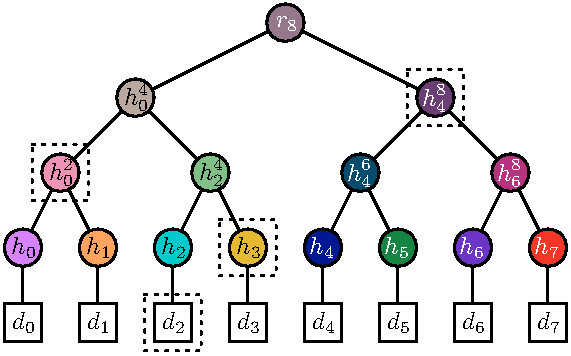
\includegraphics[width=\linewidth]{fig/mht-audit}
  %\caption{Sample Merkle hash tree with eight leaf nodes. Dashed boxes indicate
  %the nodes sent to prove the presence of the leaf $d_2$ in the tree.}
  %\label{fig:mht-audit}
%\end{figure}

%A \emph{Merkle hash tree} is a binary tree in which each leaf node's value
%represents data and each non-leaf node's value is the hash of its children's
%values~\cite{merkle1988digital}. As shown in \autoref{fig:mht-audit}, the
%structure of a Merkle hash tree allows one to efficiently prove that a data item
%is present in the tree. Specifically, given the value of the root node of the
%tree, one can verify the presence of any leaf node in the tree by computing a
%number of hashes that is logarithmic in the number of data items in the tree.

%A Merkle hash tree can store any number of nodes, i.e., the tree does not need
%to be balanced. While several ways of computing the hashes in a non-balanced
%tree exist, in this paper we use the method used in \ac{ct}~\cite{rfc6962}.
%Specifically, given $n$ items in the Merkle hash tree, let \hashfunc be a hash
%function, $d_i$ the $i$th data item (indexed from 0), and $a$ and $b$ integers
%such that $0 < a < b \le n$. Then the hash of a non-leaf node representing the
%$a$th to the $(b-1)$th data items is defined as
%\begin{equation}
  %\nodehash_a^b =
  %\begin{cases}
    %\hashfunc(0 \| d_a) & \mathrm{if\ } b = a + 1 \\
    %\hashfunc(1 \| \nodehash_a^k \| \nodehash_k^b) & \mathrm{otherwise}
  %\end{cases}
%\end{equation}
%where $\|$ denotes concatenation and $k = a + 2^{\lceil \log_2(b-a) \rceil - 1}$
%(the largest power of 2 strictly less than $b - a$). For convenience, if $b = a
%+ 1$ we write the hash as $\nodehash_a$ and call this a \emph{leaf hash}, and if
%$a = 0$ and $b = n$ then we write the hash as $r_n$ and call this the \emph{root
%hash}.

%\begin{figure}
  %\centering
  %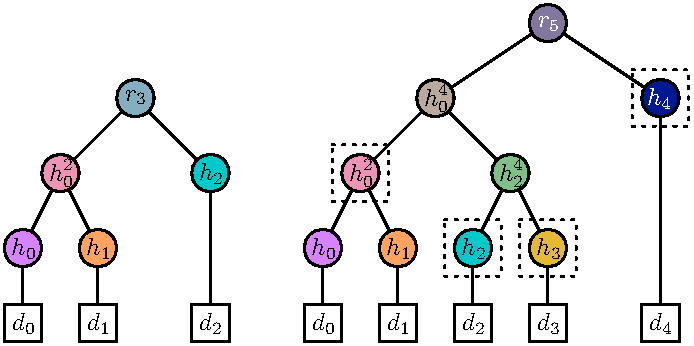
\includegraphics[width=\linewidth]{fig/mht-consistency}
  %\caption{Sample Merkle hash trees with three and five data items,
  %respectively. Dashed boxes indicate the nodes sent to prove consistency
%between the root hashes $r_3$ and $r_5$.}
  %\label{fig:mht-consistency}
%\end{figure}

%A Merkle hash tree can be used to implement an append-only, tamper-proof
%log~\cite{crosby2009efficient}. As stated above, a Merkle hash tree can provide
%an efficient \emph{proof of presence} for a given data item in the tree, thus
%proving that an item was logged. To prove that the log is append-only, that is,
%that no items have been changed or removed from the log, we can also use a
%Merkle hash tree to provide an efficient \emph{proof of consistency} that is
%logarithmic in the current size of the tree. As shown in
%\autoref{fig:mht-consistency}, a proof of consistency allows one to compute the
%root hash at two different times, thus showing that nodes have only been added
%to the tree. A tamper-proof log would periodically sign and broadcast its root
%hash, allowing clients to verify that it is not tampering with previously logged
%data.

%\steve{If we keep this subsection, describe in more detail how consistency
%proofs are formed and checked.}

%\subsection{Certificate Transparency}
%\label{sec:background:ct}

%\begin{figure}
  %\centering
  %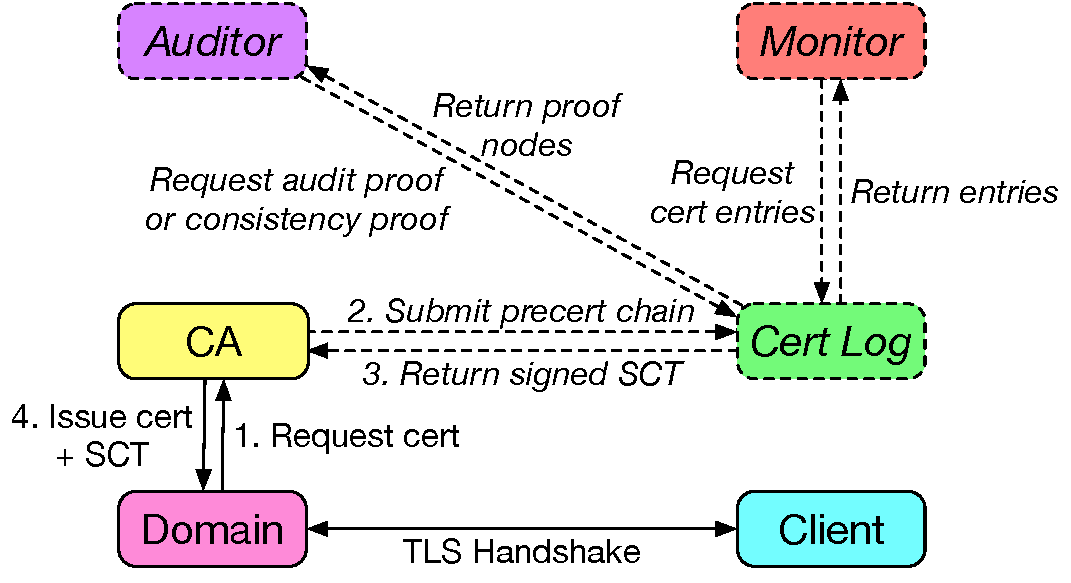
\includegraphics[width=\linewidth]{fig/ct}
  %\caption{One possible configuration of the \ac{ct} architecture. Numbered
  %steps denote the certificate issuance process. Dashed lines and boxes denote
%entities or functions introduced by \ac{ct}, with their descriptions in
%italics.}
  %\label{fig:ct}
%\end{figure}

%\acf{ct} is a project by Google focused on widespread publicization of
%certificate issuance~\cite{rfc6962}. As shown in \autoref{fig:ct}, \ac{ct}
%introduces several new roles to the \ac{ca}-based ecosystem. \emph{Certificate
%logs} are entities who record \ac{ca} behavior by maintaining a publicly
%auditable, append-only, tamper-proof database of certificates implemented using
%Merkle hash trees. \emph{Monitors} periodically retrieve these certificates to
%check for suspicious \ac{ca} behavior, such as an obscure \ac{ca} issuing a
%certificate for Google. \emph{Auditors} check for correct log behavior by
%periodically asking for \emph{audit proofs}, which show that one or more
%certificates are in a log database, or \emph{consistency proofs}, which show
%that the existing database has not been tampered with, i.e., that no certificate
%has been changed, deleted, or retroactively added to the log database.

%A log leverages Merkle hash trees to implement its certificate database. As
%explained above, the use of a Merkle hash tree allows a log to provide efficient
%proofs of presence (i.e., audit proofs) and proofs of consistency (i.e.,
%consistency proofs). While anyone may submit a certificate to a log, in current
%practice \acp{ca} usually log certificates just before issuing them, as depicted
%in \autoref{fig:ct}. Because attempting to update the Merkle hash tree in real
%time may delay or block the certificate issuance process, logs define a
%\emph{\ac{mmd}}, a time period after which a certificate is guaranteed to be
%logged, and instead return a \emph{\ac{sct}}, which is effectively a promise to
%add the certificate within the \ac{mmd}. The \ac{sct} is embedded into the
%\ac{ca}-issued certificate as an X.509 extension and used to signal that a
%domain uses \ac{ct} and that its certificate has been logged. Alternately, the
%domain can send extra information such as \acp{sct} or audit proofs in the
%\ac{tls} handshake using a \ac{tls} protocol extension. Currently, 81.9\% of
%connections that use \ac{ct} include \acp{sct} embedded as X.509 extensions,
%while 18.1\% of connections use \iac{tls} extension.

%\draft{Monitoring and auditing details. Monitors periodically downloads all new
  %entries and verifies consistency proof. Does not need to keep cert entries
  %after finishing. Auditors periodically query for random audit proofs or
  %consistency proofs. Specifically, can pass a cert hash and a size of the tree
  %and get an audit proof in return, or pass two sizes of the tree and get a
  %consistency proof in return. To verify this information, log also provides a
  %function to get the latest signed tree head. In order to detect
  %\emph{equivocation} (i.e., showing different versions of the log to different
  %queries), auditors must gossip tree heads. The log's public key is known
  %through a trusted entity such as Google.}

%\draft{\ac{ct} does not check for revocation, though multiple extensions
%designed to handle revocation have been proposed (see \autoref{sec:related}).
%Perhaps the easiest way to do to this is to create a new Merkle hash tree every
%\ac{mmd} that contains as its leaves the list of \emph{currently valid}
%certificates.}

%\subsection{Specifying and Inferring Domain Policy}
%\label{sec:background:policy}

%Previous work has proposed the use of domain-specified policies to protect
%against \ac{mitm} attacks. In AKI~\cite{kim2013accountable} and its successor
%ARPKI~\cite{basin2014arpki}, these policies are embedded within the certificates
%themselves and specify attributes such as trusted \acp{ca} and public logs as
%well as a ``cool-off period'' that forces potentially malicious certificates to
%be visible in logs for some period of time before client can accept them. In
%PoliCert~\cite{szalachowski2014policert}, the policies are stored separately in
%logs. Other work, such as Blockstack~\cite{ali2016blockstack} or
%IKP~\cite{matsumoto2017ikp}, has proposed placing policy information into a
%blockchain. While IKP's policies operate similarly to those of PoliCert,
%Blockstack simply provides the domain's keys directly. Of these proposals, only
%ARPKI leverages the relationship between \acp{ca} and logs to ease the burden on
%the domain during certificate issuance, but all proposals require the domain to
%specify its policy in detail to prevent \ac{mitm} attacks resulting from
%misbehaving \acp{ca}. \steve{TODO: describe drawbacks in more detail once the
%arguments are more developed}

%There has also been some work that takes a heuristic approach, using the past
%behavior of \acp{ca} in order to determine how clients should trust them. For
%example, CAge~\cite{kasten2013cage} propose a system that displays a browser
%warning to users for certificates whose names are under a DNS top-level domain
%that the issuing \ac{ca} has never signed for before. Perl, Fahl and Smith
%propose to outright remove root certificates that have not been used to sign
%(either directly or through \ac{ca} delegation) any observed certificates in the
%past~\cite{perl2014you}. Both of these proposals use data from
%Censys~\cite{durumeric2015search} or its predecessors, but do not use any
%information from the domains themselves. Because of this, these approaches may
%encounter situations where they mistake a legitimate, domain-initiated change
%with an attempted \ac{mitm} attack and thus block a user from visiting a benign
%site or expose a user to the \ac{mitm} attack. Indeed, a previous study of
%changes in the Web \ac{pki}'s trust graph suggests that legitimate changes and
%attacks share properties to the point that they cannot be easily
%distinguished~\cite{amann2013no}.

%\subsection{Signaling \ac{https} Deployment}
%\label{sec:background:signaling}

%Although \ac{hsts}~\cite{rfc6797} enforces the use of \ac{https} for a site
%after a client has connected with that site over \ac{https} for the first time,
%previous work has acknowledged the difficulty (in terms of both storage and
%latency overhead) of identifying \ac{https}-deploying domains before the first
%visit. The prevailing solution among browser vendors is \emph{\ac{hsts}
%preloading}~\cite{keeler2012preloading}, in which browser vendors include a list
%of the most popular sites that have deployed \ac{https}. These lists are
%incomplete (covering only \steve{TODO: fill in} names in Chrome), and domains
%must explicitly opt into adding themselves. As indicated by vendor-provided
%guidelines,\footnote{\url{https://hstspreload.org/}} this process is prone to
%mistakes by domain operators that lead to site inaccessibility.

%As described in \steve{TODO: refer to previous section if mentioned elsewhere},
%most approaches to disseminating certificate revocation information fail for
%signaling because they rely on assumptions that do not hold in the signaling
%problem. In particular, the use of \acp{crl}~\cite{rfc5280} does not scale to
%the number of \ac{https}-deploying sites because we cannot assume that the
%number of sites deploying \ac{https} will remain small compared to the overall
%number of sites. More efficient versions of \acp{crl} also do not work: an
%approach similar to Chrome's CRLsets~\cite{langley2012revocation} suffers from
%the same incompleteness and opt-in hurdles mentioned above, and an approach
%similar to CRLite~\cite{larisch2017crlite} relies on knowledge of all domain
%names, which is infeasible in today's DNS due to many country code top-level
%domains keeping their registries private. Approaches such as storing data in a
%2-3 tree~\cite{naor1998certificate} or aoptimized Merkle hash
%tree~\cite{laurie2012revocation}, while able to provide efficient proofs of
%\ac{https} deployment, require online checks by clients, greatly increasing the
%latency of connection establishment.

%DANE~\cite{rfc6698}, which uses DNS to send a public key, certificate, or
%\ac{ca} that the client should expect, can provide both signaling and policy
%management with little added latency and without requiring browsers to store any
%kind of signaling information. However, DANE relies on DNSSEC~\cite{rfc4033},
%and both have a low deployment rate in today's Internet. Since DANE's
%standardization in 2011 and DNSSEC's in 2005, only 5,885 DANE records for
%\ac{https} and 1.67M verified DNSSEC zones out of more than 329M registered DNS
%names overall~\cite{dnib-14-1}
%exist.\footnote{\url{http://secspider.verisignlabs.com/stats.html}, retrieved 1
%August 2017} Changing these numbers would require significant deployment efforts
%on the parts of domains, including registering domain names through the subset
%of DNS registrars that offer DNSSEC, usually as a paid service.
